\chapter{Run-Time Monitoring}
\label{chap:monitoring}

Run-time monitoring techniques have been shown to be useful for improving the
reliability, security, and debugging capabilities of computer systems. For
example, Hardbound is a hardware-assisted technique to detect out-of-bound
memory accesses, which can cause undesired behavior or create a security
vulnerability if uncaught \cite{hardbound-asplos08}.  Intel has recently
announced plans to support buffer overflow protection similar to Hardbound in
future architectures \cite{intel-mpx}. Similarly, run-time monitoring can
enable many other new security, reliability, and debugging capabilities such as
fine-grained memory protection \cite{mondrian-asplos02}, information flow
tracking \cite{dift-asplos04, testudo-micro08}, hardware error detection
\cite{argus-micro07}, data-race detection \cite{radish-isca12, cord-hpca06},
etc. 

In this section, we cover background information on run-time monitoring.
Section~\ref{chap:monitoring.overview} covers terminology and our model of
run-time monitoring. Section~\ref{chap:monitoring.techniques} discusses some
example monitoring techniques in detail.

\section{Overview}
\label{chap:monitoring.overview}


% Previous work overheads
\begin{table*}[t]
  \begin{center}
    \vspace{-0.0in}
    \begin{tiny}
    %\begin{tabular}{|l|p{2in}|r|r|}
\begin{tabular}{|l|l|l|r|}

\hline
{\bf Name} & {\bf Type} & {\bf Monitoring scheme and flexibility} & {\bf Slowdown (avg./worst)} \\ \hline\hline

% DIFT \cite{dift-asplos04} & Custom HW & DIFT only & 1.1\% / 23\% \\ \hline
% FlexiTaint \cite{flexitaint-hpca08} & Custom HW & DIFT w/ programmable policies & 1.1\%-3.7\% / 8.7\% \\ \hline
% Hardbound \cite{hardbound-asplos08} & Custom HW & Array bounds checks only & 5\%-9\% / 22\% \\ \hline
% Harmoni \cite{harmoni-dsn12} & Custom HW & Tag-based monitors & 1\%-10\% / 20\% \\ \hline\hline

DIFT \cite{dift-asplos04} & Custom HW & DIFT only & 1.01x / 1.23x \\ \hline
FlexiTaint \cite{flexitaint-hpca08} & Custom HW & DIFT w/ programmable policies & 1.01x-1.04x / 1.09x \\ \hline
Hardbound \cite{hardbound-asplos08} & Custom HW & Array bounds checks only & 1.05x-1.09x / 1.22x \\ \hline
Harmoni \cite{harmoni-dsn12} & Custom HW & Tag-based monitors & 1.01x-1.10x / 1.20x \\ \hline\hline

FlexCore \cite{flexcore-micro10} & Dedicated FPGA & Instruction-trace monitoring & 1.05x-1.44x / 1.84x \\ \hline
FADE \cite{fade-hpca14} & Core+Custom HW & Instruction-trace monitoring (effective when HW filters work) & 1.2x-1.8x / 3.3x \\ \hline
LBA-accelerated \cite{lba-isca08} & Multi-core+Custom HW & Instruction-trace monitoring (effective when accelerators work) & 1.02x-3.27x / 5x \\ \hline
LBA \cite{lba-asid06} & Multi-core+Custom HW & Instruction trace monitoring & 3.23x-7.80x / 11x \\ \hline \hline

Multi-core DIFT \cite{nagarajan-interact08} & SW (multithreaded) & DIFT (compiled for each application) & 1.48x / 2.2x \\ \hline

LIFT \cite{lift-micro06} & SW (DBI) & DIFT (fully flexible) & 3.6x / 7.9x \\ \hline
Purfiy \cite{purify-usenix92} & SW (DBI) & Memory leak checks (fully flexible) & 2.3x / 5.5x \\ \hline
TaintCheck \cite{taintcheck-ndsss05} & SW (DBI) & DIFT (fully flexible) & 10x / 27x \\ \hline


\end{tabular}

    \end{tiny}
    \caption{Trade-off between performance overhead and flexibility/complexity of run-time monitoring systems.}
    \vspace{-0.2in}
    \label{tab:monitoring.previous_overheads}
  \end{center}
\end{table*}

\textbf{[Hardware vs. software implementations vs. configurable hardware]}
There have been a number of proposals for run-time monitoring systems exploring
various design points. % in the trade-off space between efficiency and
flexibility.  Table~\ref{tab:monitoring.previous_overheads} summarizes some of
the representative designs and their reported performance overhead. The
previous studies clearly show that there exist trade-offs between efficiency,
flexibility, and hardware costs.  For example, a run-time monitoring scheme can
often be realized with fairly low performance overhead (less than 20\%) if
implemented with custom hardware that is designed only for one monitor or a
narrow set of monitors. However, the custom hardware monitors cannot be
modified or updated, and require dedicated silicon area.  On the other hand,
flexible systems that support a wide range of monitors lead to noticeable
performance overhead, often too high for wide deployment in practice.
Software-only implementations \cite{nagarajan-interact08, lift-micro06,
purify-usenix92, taintcheck-ndsss05} or multi-core monitors with minimal
hardware changes \cite{lba-asid06} are reported to have severalfold slowdowns.
On-chip FPGA monitors \cite{flexcore-micro10} and cores with monitoring
accelerators \cite{lba-isca08, fade-hpca14} can reduce overhead significantly,
but still show slowdowns of several tens of percents in some cases.  In today's
monitoring systems, the overheads are also unpredictable because they depend
heavily on the characteristics of applications and monitoring operations.  In
summary, users currently need to either pay noticeable overhead or the cost of
custom hardware in order to use fine-grained run-time monitoring in deployed
systems.

% Run-time monitoring overview
\begin{figure}
  \begin{center}
    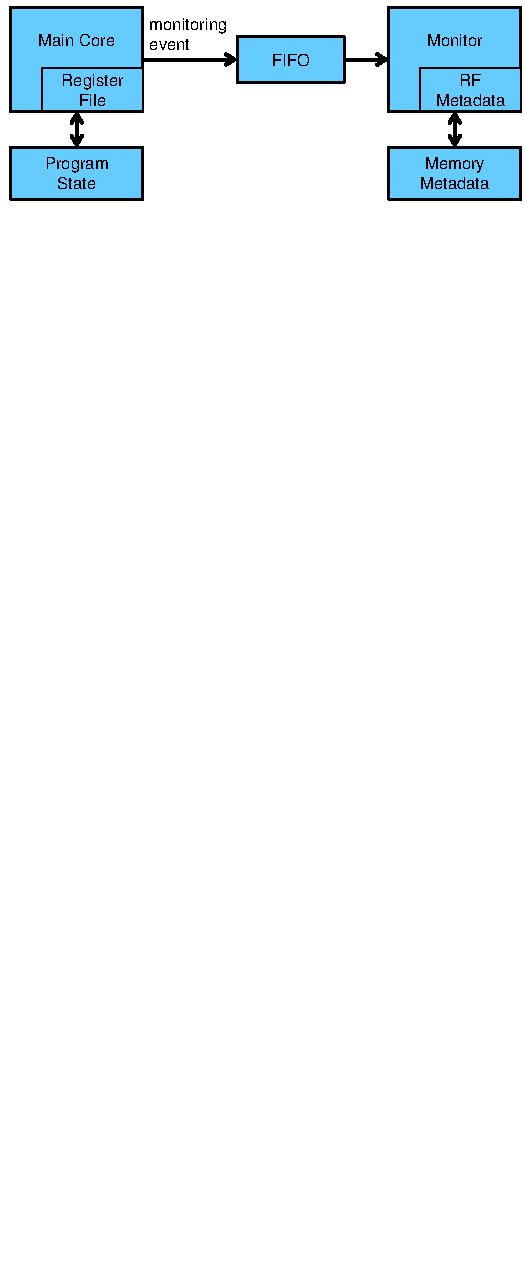
\includegraphics{figs/monitoring_architecture.pdf}
    \vspace{-0.2in}
    \caption{Overview of run-time monitoring architecture.}
    \label{fig:monitoring.overview} 
    \vspace{-0.1in}
  \end{center}
\end{figure}

\textbf{[Model of monitoring]}
Figure~\ref{fig:monitoring.overview} shows an overview of the run-time monitoring
model that is assumed in this paper.  The \emph{main program} is a computation
task that performs the original function of the system and is run on the
\emph{main core}.  On certain events during the main program, such as the
execution of certain types of instructions, the \emph{monitor} performs a
series of \emph{monitoring operations}. The monitor operates in parallel to the
main core. Events that trigger monitoring are referred to as \emph{monitoring
events}. Depending on the type of monitoring event, different monitoring
operations are executed. Information about monitoring events is sent to the
monitor and buffered in a FIFO structure to decouple the running of the main
core and the monitor. If the FIFO is full, then the main core is forced to
stall on a monitoring event until a FIFO entry becomes available. These stalls
are a major source of overhead because the monitor may take several cycles to
process a single event from the main core.  Monitors typically maintain
metadata corresponding to each memory location ({\tt mem\_metadata[addr]}) and
register ({\tt rf\_metadata[reg\_id]}) of the main core.  If the monitor
detects an inconsistent or undesired behavior in the monitoring events, then an
error is detected. 

There are many possible monitoring schemes that can be implemented on this type
of fine-grained parallel monitoring architecture such as memory protection
\cite{mondrian-asplos02}, information flow tracking \cite{dift-asplos04,
testudo-micro08}, soft error detection \cite{argus-micro07}, data-race
detection \cite{cord-hpca06, eraser-tocs97, literace-pldi09, pacer-pldi10}, etc.  For example, an array bounds
check (BC) \cite{hardbound-asplos08} can be implemented in order to detect when
software attempts to read or write to a memory location outside of an array's
bounds. This can be done by associating metadata with array pointers that
indicates the array's base (start) and bound (end) addresses. On loads or
stores with the array pointer, the monitor checks that the memory address
accessed is within the base and bound addresses. In addition, this base and
bound metadata is propagated on ALU and memory instructions to track the
corresponding array pointers.

\section{Monitoring Techniques}
\label{chap:monitoring.techniques}

\subsection{Array Bounds Check}

% Example monitor
\begin{figure*}
  \begin{center}
    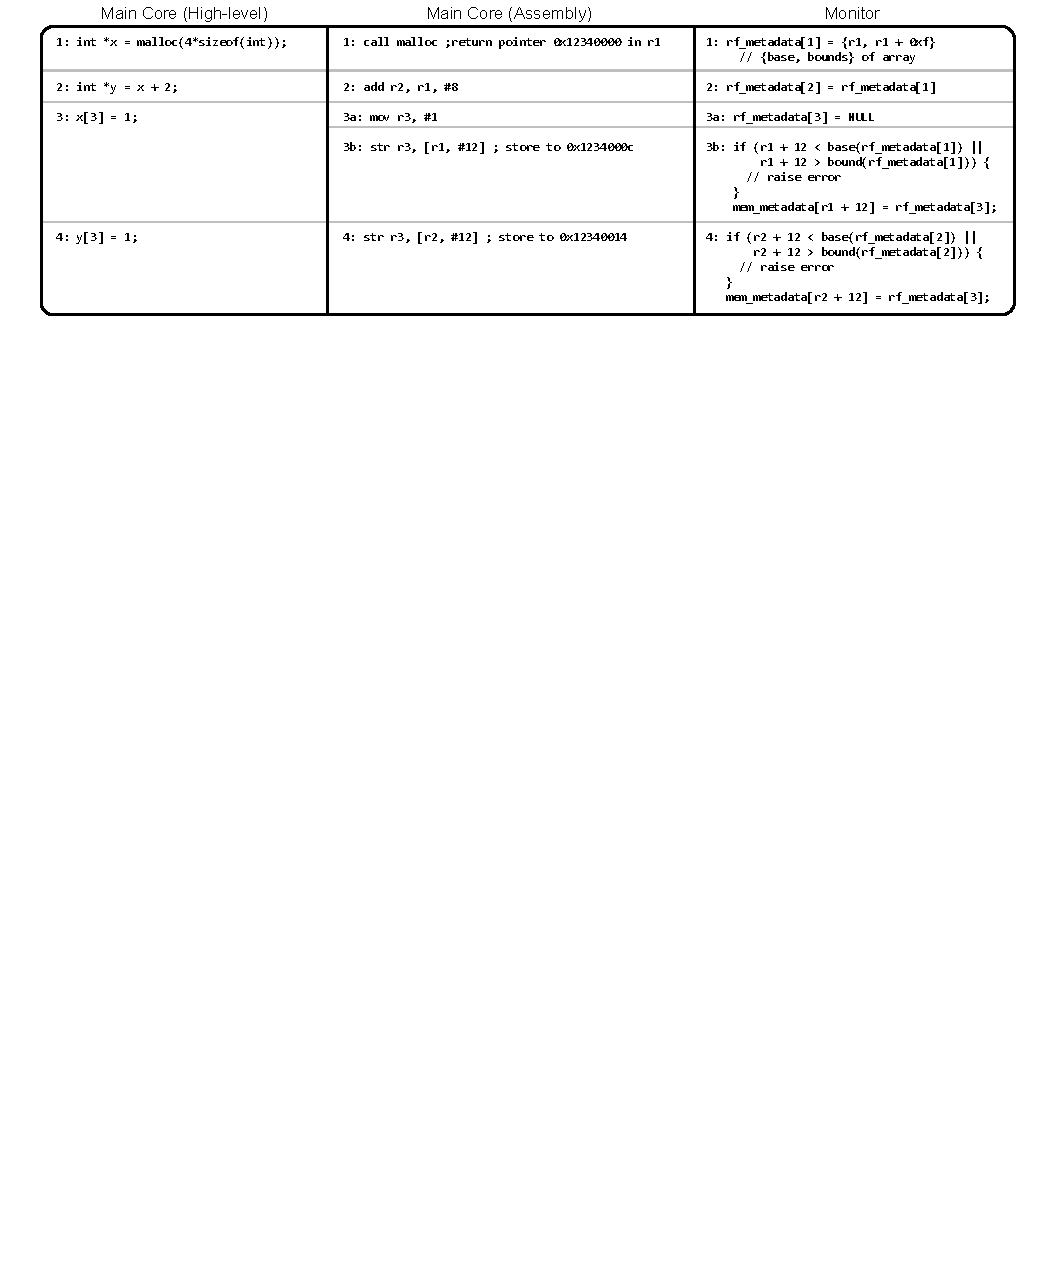
\includegraphics[width=\columnwidth]{figs/code_bc.pdf}
    \caption{Example of array bounds check monitor.}
    \label{fig:monitoring.code_bc}
    \vspace{-0.1in}
  \end{center}
\end{figure*} 

Figure~\ref{fig:monitoring.code_bc} shows an example pseudo-code segment,
its assembly level instructions, and the corresponding monitoring operations
for an array bounds check monitor. 
First, an array {\tt x} is allocated using {\tt malloc} (line 1). 
As {\tt malloc} returns the array's address in a register, the monitor
associates base and bounds metadata with the corresponding register. 
Next, pointer {\tt y} is set to point to the middle of array {\tt x} (line 2). 
At the assembly level, a register {\tt r2} is set to array {\tt x}'s address plus an offset.
The monitor propagates the metadata of the original pointer in {\tt r1} to the
metadata of {\tt r2}. This is to ensure that pointer {\tt y} is not used to exceed the array's bounds.
Line 3a shows setting register {\tt r3} to a constant value of 1.
When this happens,
{\tt r3}'s metadata is reset to NULL in case it previously stored a
pointer. 
Finally, the value of {\tt r3} is written to memory using both pointers {\tt x} and {\tt y}.
In both cases, the monitor checks whether the store address is within the bounds of the register metadata. In the first case (line 3b), {\tt x+12}
is within the original array's bounds. No error is raised and the metadata of
{\tt r3} is propagated to the metadata of the store address. If {\tt r3} were a
pointer, then this would allow a future instruction to load the pointer and use
it to access the corresponding array or data structure. In the second case,
{\tt y+12} (line 4) corresponds to {\tt x+20} which is not within the array's bounds and
the monitor will raise an error. 

Note that this monitoring is performed automatically and transparently with
almost no modification needed to the main program. The only modification to
the main program that is needed is to initially set metadata, such as setting
the base and bounds addresses on a {\tt malloc} call for array bounds check.
The propagation and checks of the metadata occur automatically as
instructions are forwarded.
Here, we have shown the dynamic sequence of operations executed by the monitor but
the actual static code consists of a set of instructions to be run for each
possible instruction type (load, store, etc.). Only instruction types relevant
for the particular monitoring scheme are forwarded.



\subsection{Dynamic Information Flow Tracking}

\subsection{Uninitialized Memory Check}

